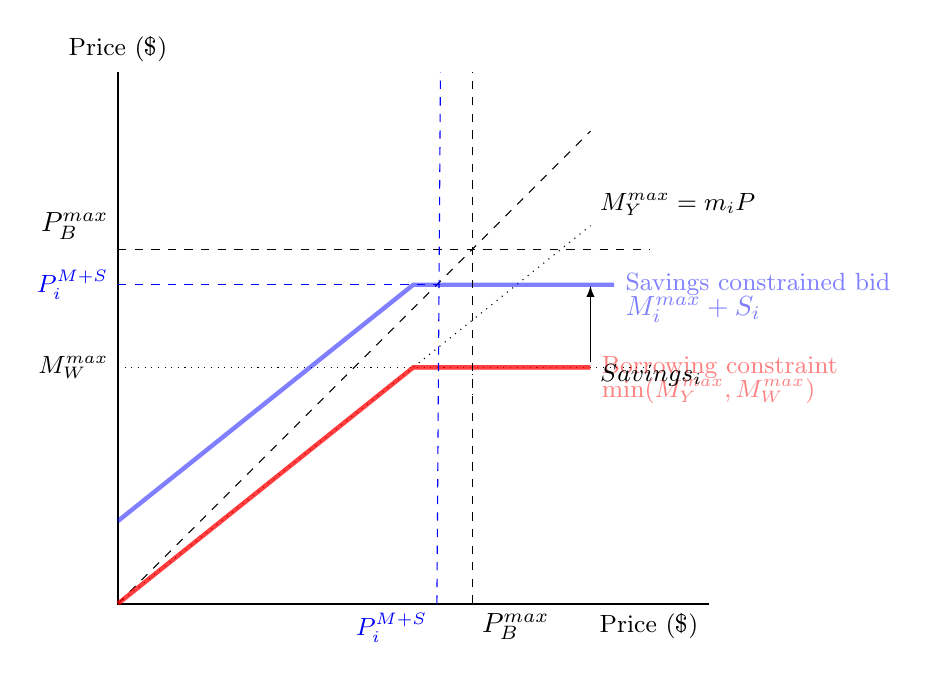
\begin{tikzpicture}	[scale=1.5]
%AXES
\draw[thick] (0,4.5)node[above]{\small Price (\$)} --(0,0)--(5,0)node[below left]{\small Price (\$)};
%\node at (-.25, 3.5)[ rotate=90]{\small Mortgage, Price (\$)};
% M =Mi MAX
\draw[dashed] (0,0)--(4,4);{node[right]}; %{\small $P$};
\draw[dotted] (0,2)node[left]{\small $M_W^{max}$}--(4.5,2);%node[right, red]{\small $M = M_i^{max}$};
% M =mi MAX
%\draw[dotted,red, opacity=.5] (0,0)--(4,3.6)node[right]{\small $M = 0.9P$};
\draw[dotted] (0,0)--(4,3.2)node[above right]{\small $M^{max}_Y = m_iP$};
% COMBINED MAX RED
\draw[ultra thick, red, opacity=.5] (0,0)--(2.5,2)--(4.0,2)node[right]{\small Borrowing constraint};
\draw[ultra thick, red, opacity=.5] (0,0)--(2.5,2)--(4.0,2)node[below right]{\small min($M_{Y}^{max},M_{W}^{max}$) };

\draw[ultra thick, blue, opacity=.5] (0,.7)--(2.5,2.7)--(4.2,2.7)node[right, ]{\small Savings constrained bid}node[below right, ]{$M_i^{max}+S_i$};
% SAVINGS
\draw[-latex] (4,2.05)node[below=5, right] {\small $Savings_i$}--(4,2.69);
% PMAX
\draw[dashed, ] (3,0)node[below right] {$P_B^{max}$}--(3,4.5);%node[, right]{\small desired max bid};
\draw[dashed,] (0,3)node[above left] {$P_B^{max}$}--(4.5,3);%node[, right]{\small desired max bid};

\draw[dashed, blue, thin] (2.7,0)node[below left] {\small $P_i^{M+S}$}--(2.73,4.5); %node[left, text width= 2cm]; %{\small };
\draw[blue, thin, dashed] (0,2.7)node[left] {\small $P_i^{M+S}$}--(2.73,2.7);%node[left, text width= 2cm]{\small savings constrained bid};
\draw[dotted ] (3,2)--(3,1.72);
\end{tikzpicture}